%% LyX 2.2.3 created this file.  For more info, see http://www.lyx.org/.
%% Do not edit unless you really know what you are doing.
\documentclass[english]{article}
\usepackage[T1]{fontenc}
\usepackage[latin9]{inputenc}
\usepackage{geometry}
\geometry{verbose,tmargin=2cm,bmargin=2cm,lmargin=2cm,rmargin=2cm,headheight=2cm,headsep=2cm}
\setlength{\parindent}{0bp}
\usepackage{float}
\usepackage{textcomp}
\usepackage{graphicx}
\usepackage{babel}
\begin{document}

\section*{Ejercicio 3: Simulaci�n de la respuesta en frecuencia de un circuito
en condiciones iniciales}

Durante este ejercicio se procedi� a simular el circuito de la Figura
\ref{c_3}. Se nos pidi� obtener que tipo de singularidad era el circuito,
a que elemento reactivo se asociaba, y cual valor era el que deb�a
ser ese elemento. Al realizar la simulaci�n, se obtuvo un Bode como
el que se puede ver en la figura \ref{b_3}.

\begin{figure}[H]
\begin{centering}
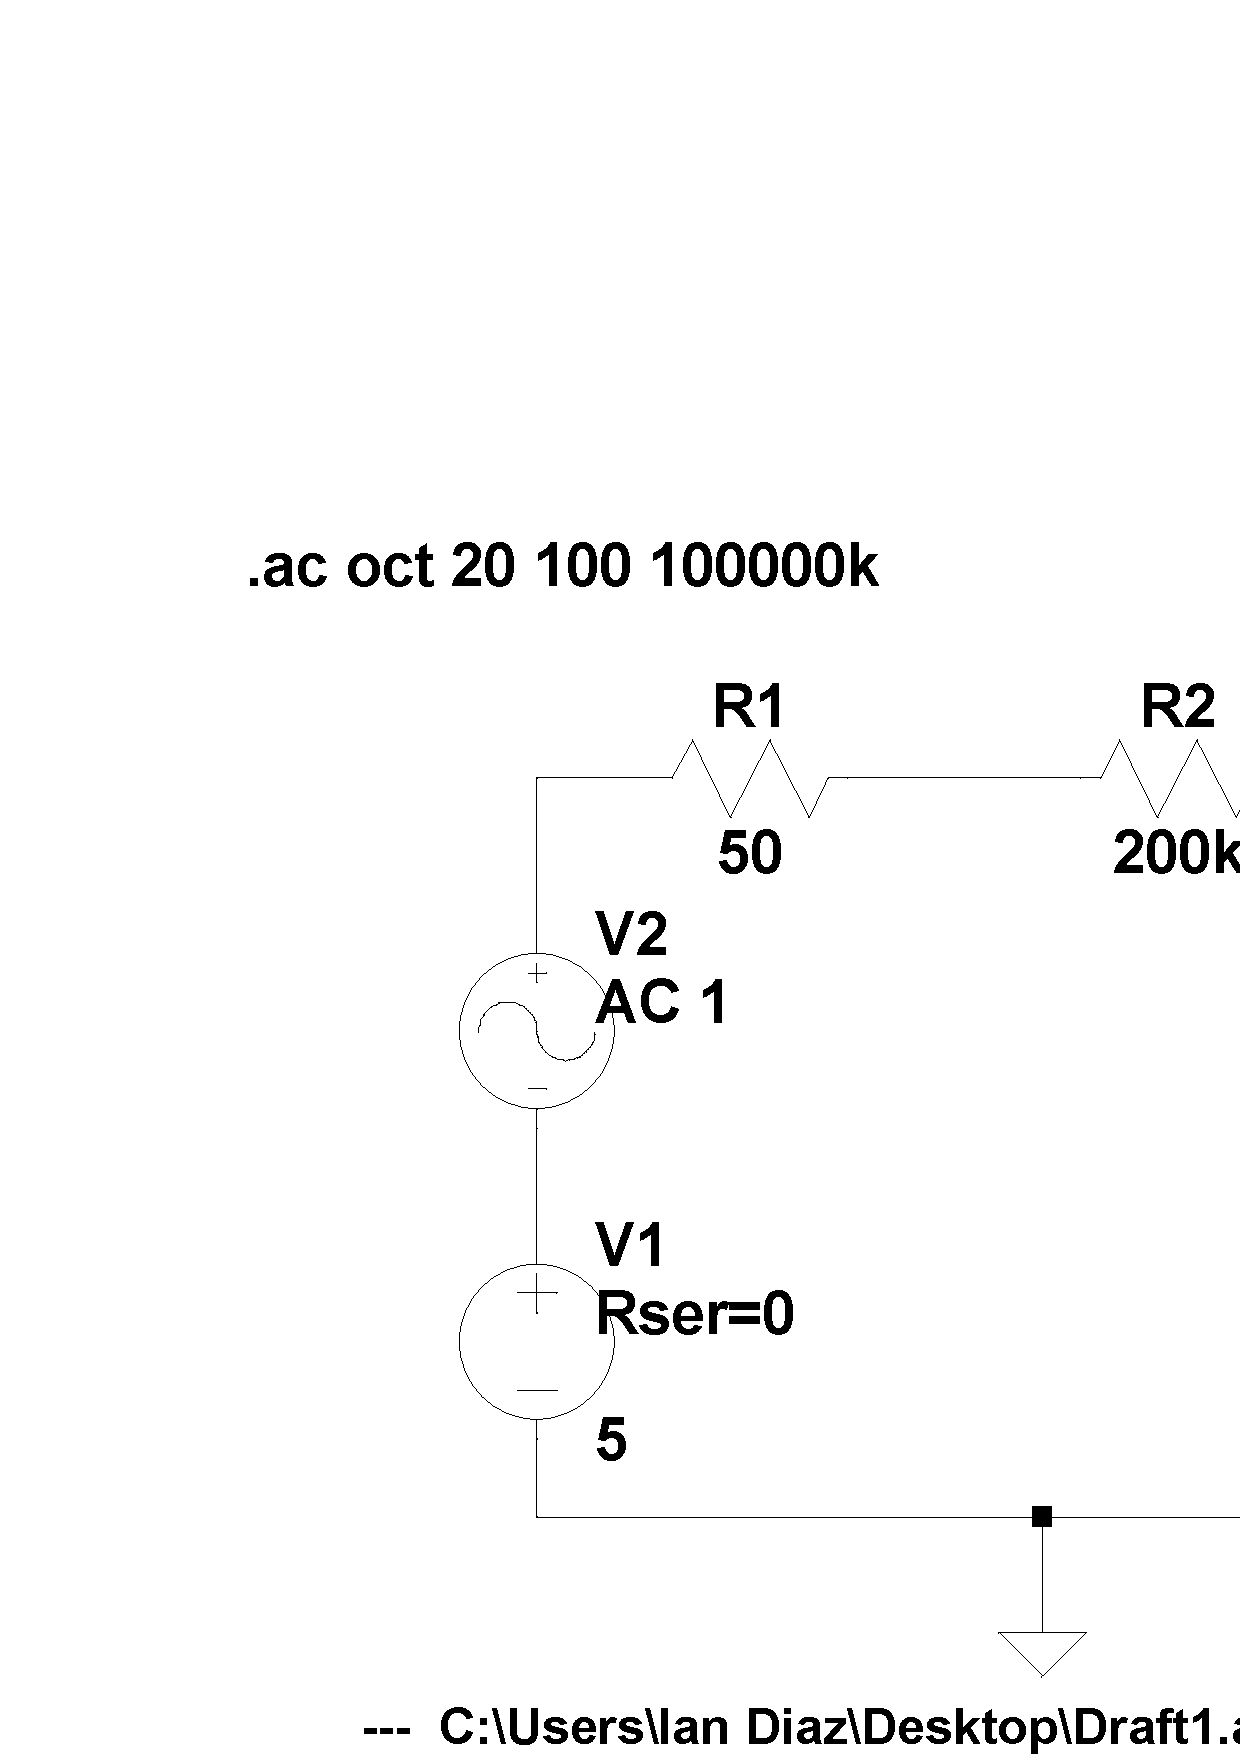
\includegraphics[scale=0.2]{Circuit}
\par\end{centering}
\caption{Circuito}
\label{c_3}

\end{figure}

\begin{figure}[H]
\begin{centering}
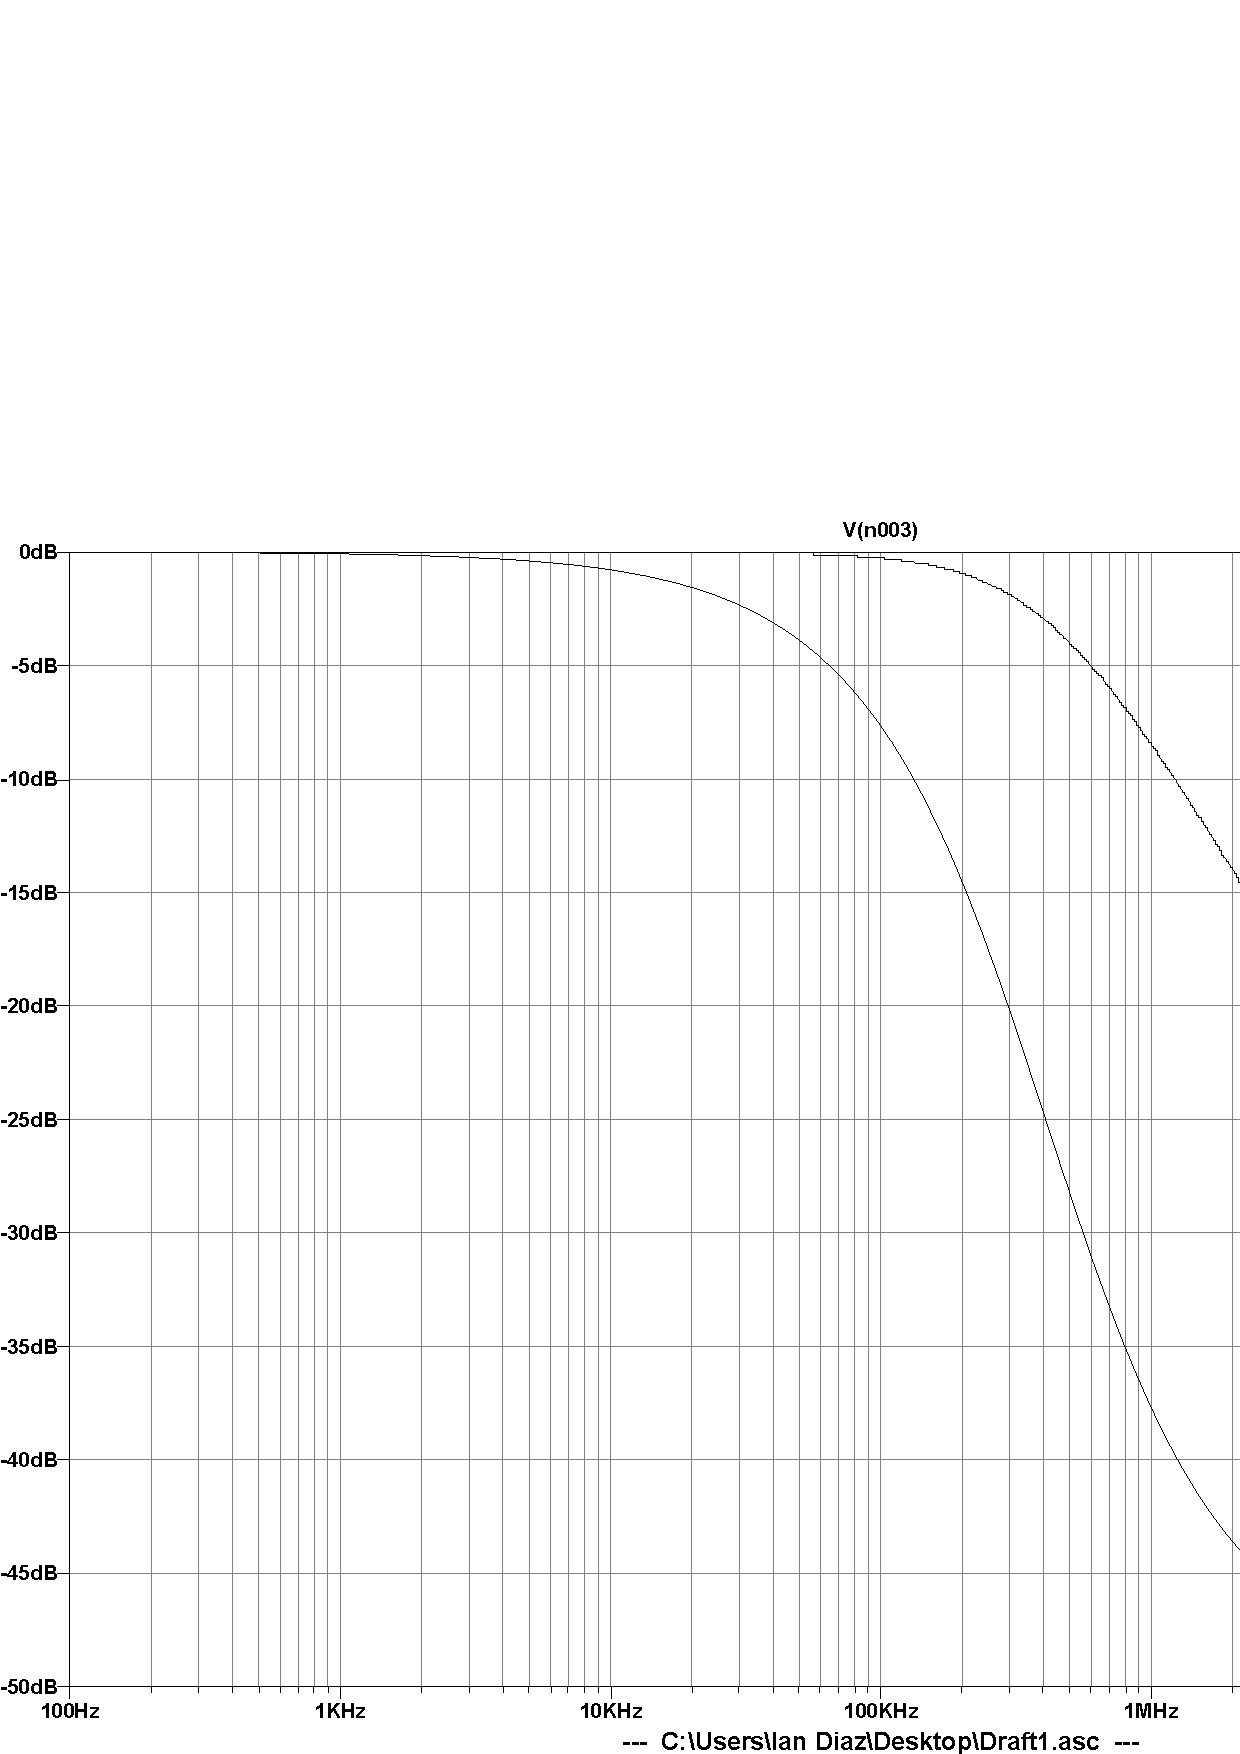
\includegraphics[scale=0.25]{Bode}
\par\end{centering}
\caption{Bode}
\label{b_3}

\end{figure}

Viendo el bode de la figura \ref{b_3}, sabiendo que la amplitud es
la linea negra y la fase la linea gris, podemos determinar que se
comporta como un pasabajos y es un polo, ya que la fase cae 90\textdegree .
Por lo tanto, podemos decir que diodo, a altas frecuencias se comporta
como un capacitor. Luego de ver este comportamiento, buscamos la hoja
de datos del 1N4148 y se encontro que la capacidad total del diodo
es de 4(pF), sin embargo, como se puede ver en la figura \ref{b2_3},
el bode no coincide completamente con el del circuito de la figura
\ref{c_3}. Para que coincida perfectamente, debemos usar un capacitor
de aproximadamente 2(pF). Creemos que la diferencia de capacidad entre
el valor obtenido en la hoja de datos y e calculado, se debe a un
modelo equivalente del diodo que no se coincide exactamente con el
de la realidad, generando peque�as diferencias como esta.

\begin{figure}[H]
\begin{centering}
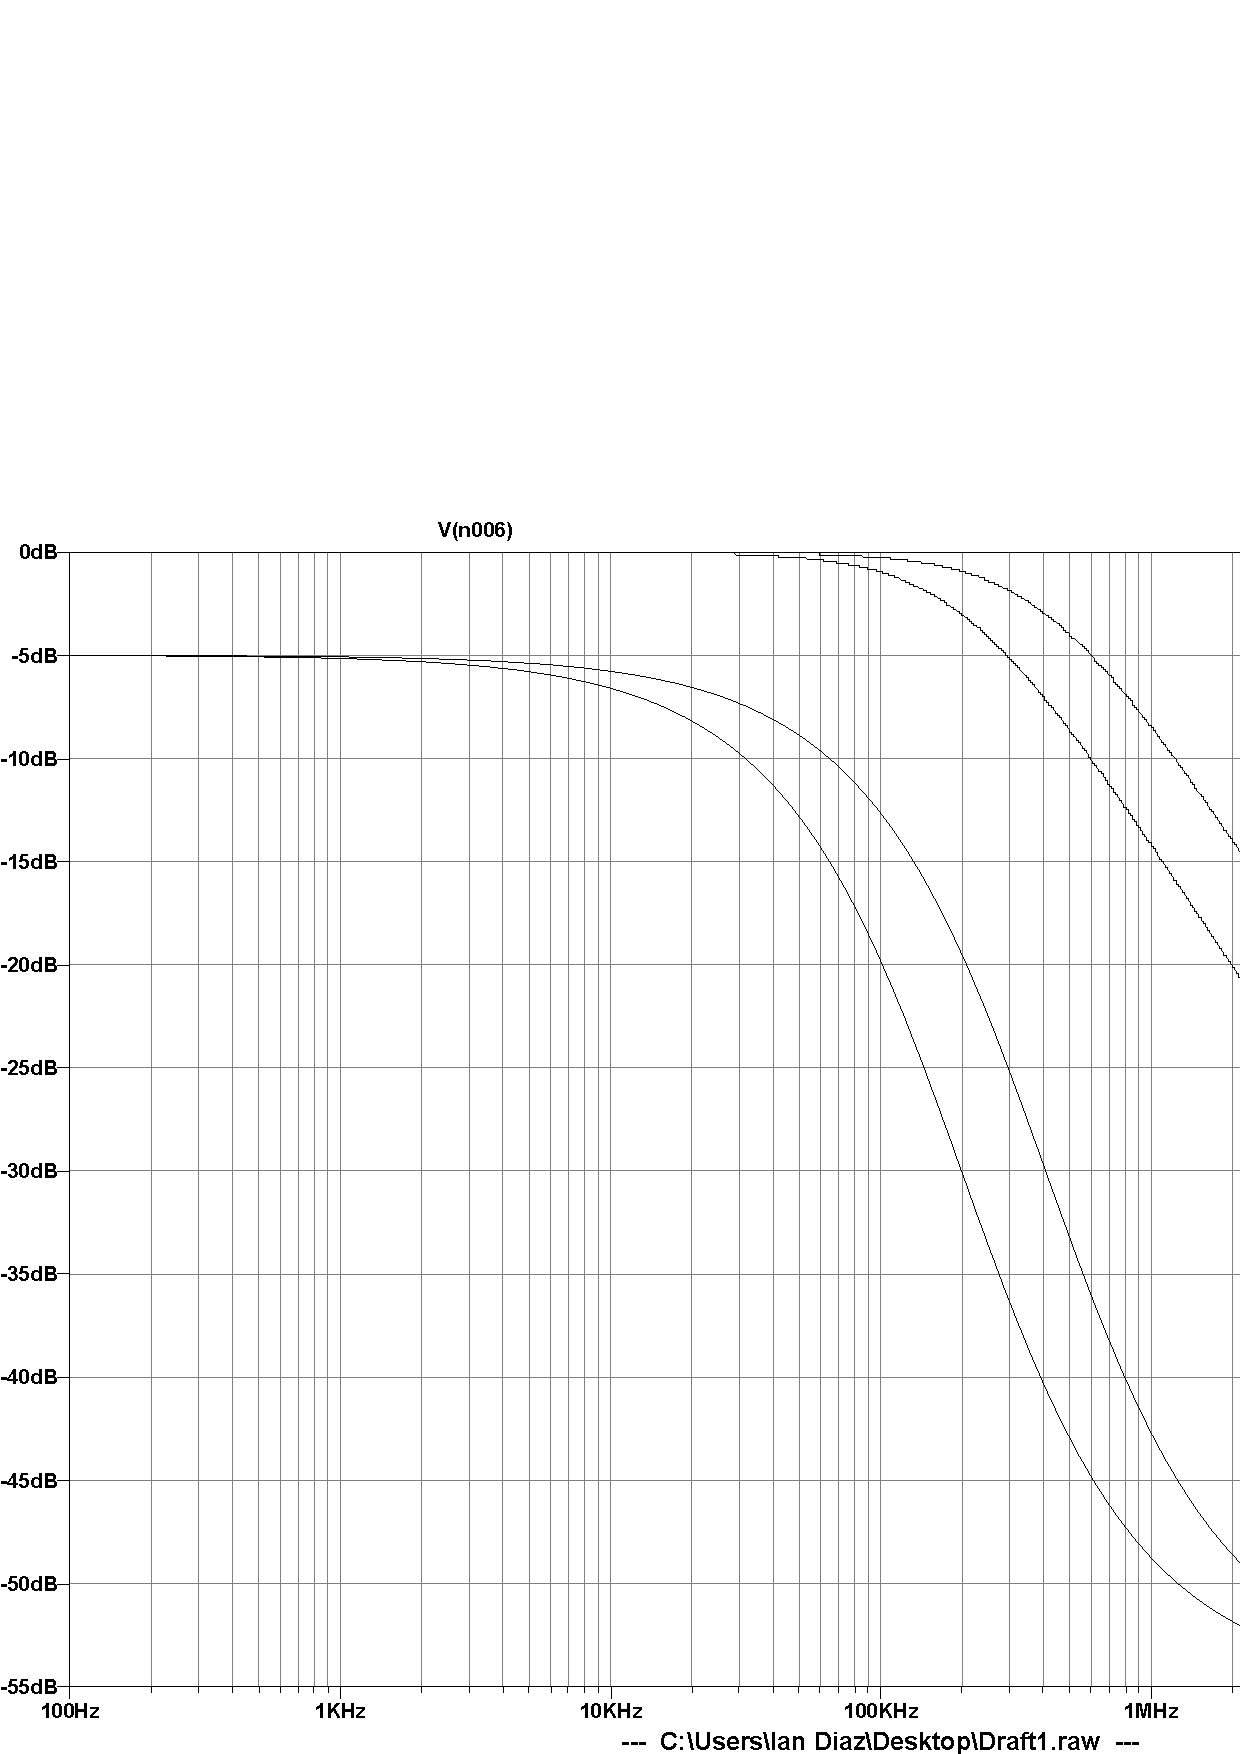
\includegraphics[scale=0.2]{Bode2}
\par\end{centering}
\caption{Bode Diodo vs Capacitor nominal}

\label{b2_3}
\end{figure}

\end{document}
